% METADATA SUBSTRATE DESIGN VISUALS
% As-built architecture of the metadata stack + its four consumers,
% generated for deep technical review. Same visual language as
% STS2_DESIGN_VISUALS_V2.tex (sqltoolsservice/refactor_docs).
% Compile: pdflatex METADATA_DESIGN_VISUALS.tex (twice)
% NOTE: authored without local TeX tooling — if a page overflows,
% the enclosing \adjustbox scales it; report any compile error and
% it will be a small bracket/typo fix, not a structural one.
\documentclass[10pt]{article}
\usepackage[a4paper,landscape,margin=10mm]{geometry}
\usepackage[T1]{fontenc}
\usepackage[sc]{mathpazo}
\usepackage{microtype}
\usepackage{tikz}
\usetikzlibrary{arrows.meta,positioning,fit,calc,backgrounds,shapes.geometric,shapes.multipart,decorations.pathreplacing,matrix}
\usepackage{xcolor}
\usepackage{adjustbox}
\usepackage{hyperref}
\hypersetup{hidelinks}
\pagestyle{empty}
\setlength{\parindent}{0pt}

\definecolor{runtime}{HTML}{EAF0FF}   % store / registry layer
\definecolor{core}{HTML}{EAF8EC}      % pure snapshot / pure consumers
\definecolor{journal}{HTML}{FFF0EE}   % sessions / data plane
\definecolor{observer}{HTML}{F6EDFA}  % observability
\definecolor{edge}{HTML}{FFF5E6}      % engine / hydration
\definecolor{external}{HTML}{F4F4F4}  % external systems
\definecolor{risk}{HTML}{FFE3E3}
\definecolor{good}{HTML}{E2F5E7}
\definecolor{policy}{HTML}{E8F7F5}    % privacy / honesty gates
\definecolor{ink}{HTML}{263238}
\definecolor{muted}{HTML}{607D8B}
\definecolor{blue}{HTML}{3F6FB5}
\definecolor{red}{HTML}{B54A4A}
\definecolor{purple}{HTML}{7A4E9B}
\definecolor{orange}{HTML}{B56A24}
\definecolor{green}{HTML}{39784A}

\tikzset{
  >=Latex,
  every node/.style={font=\small,text=ink},
  box/.style={draw=ink!65,rounded corners=2.5pt,fill=runtime,minimum height=11mm,minimum width=35mm,align=center,inner sep=4pt},
  corebox/.style={box,fill=core},
  sessbox/.style={box,fill=journal,draw=red!75},
  obsbox/.style={box,fill=observer,draw=purple!70},
  enginebox/.style={box,fill=edge,draw=orange!75},
  extbox/.style={box,fill=external,dashed},
  policybox/.style={box,fill=policy,draw=green!70},
  riskbox/.style={box,fill=risk,draw=red!80},
  goodbox/.style={box,fill=good,draw=green!75},
  tinybox/.style={draw=ink!60,rounded corners=2pt,fill=white,align=center,inner sep=3pt,font=\footnotesize},
  state/.style={draw=ink!65,rounded corners=6pt,fill=runtime,minimum width=29mm,minimum height=10mm,align=center},
  term/.style={state,fill=good},
  badstate/.style={state,fill=risk,draw=red!80},
  arrow/.style={->,very thick,draw=ink!75},
  async/.style={->,thick,dashed,draw=purple},
  write/.style={->,very thick,draw=red},
  effect/.style={->,very thick,draw=orange},
  policyarr/.style={->,very thick,draw=green},
  fail/.style={->,very thick,dashed,draw=red},
  note/.style={draw=ink!30,rounded corners=2pt,fill=white,align=left,inner sep=5pt,font=\footnotesize,text width=70mm},
  pill/.style={draw=ink!45,rounded corners=7pt,fill=white,inner xsep=6pt,inner ysep=2pt,font=\footnotesize\bfseries},
  label/.style={font=\footnotesize,align=center,fill=white,inner sep=1.5pt},
}
\newcommand{\code}[1]{\texttt{#1}}
\newcommand{\pagehead}[2]{%
  \begin{minipage}[t]{0.73\linewidth}
    {\Large\bfseries #1}\\[-1mm]
    {\small\color{muted}#2}
  \end{minipage}\hfill
  \begin{minipage}[t]{0.25\linewidth}\raggedleft
    {\footnotesize Metadata substrate --- as-built design}\\
    {\scriptsize vscode-mssql 99a44957c $\cdot$ sqltoolsservice 7532d145}
  \end{minipage}
  \vspace{3mm}\hrule\vspace{4mm}
}
\newcommand{\legend}{%
\tikz[baseline=-0.7ex]\node[box,minimum width=7mm,minimum height=4mm,inner sep=1pt]{}; store/registry\quad
\tikz[baseline=-0.7ex]\node[corebox,minimum width=7mm,minimum height=4mm,inner sep=1pt]{}; pure snapshot\quad
\tikz[baseline=-0.7ex]\node[enginebox,minimum width=7mm,minimum height=4mm,inner sep=1pt]{}; engine/hydration\quad
\tikz[baseline=-0.7ex]\node[sessbox,minimum width=7mm,minimum height=4mm,inner sep=1pt]{}; sessions/data plane\quad
\tikz[baseline=-0.7ex]\node[policybox,minimum width=7mm,minimum height=4mm,inner sep=1pt]{}; honesty/privacy gate\quad
\tikz[baseline=-0.7ex]\node[obsbox,minimum width=7mm,minimum height=4mm,inner sep=1pt]{}; observability
}

\begin{document}

% =====================================================================
% PAGE 1 — LAYERED ARCHITECTURE
% =====================================================================
\pagehead{1. The metadata stack and its four consumers}
{Three layers (snapshot / engine / store) under two narrow seams; every consumer pins once per response and renders failure as failure.}
\legend\par\vspace{4mm}

\begin{adjustbox}{max width=\linewidth,max height=0.82\textheight,center}
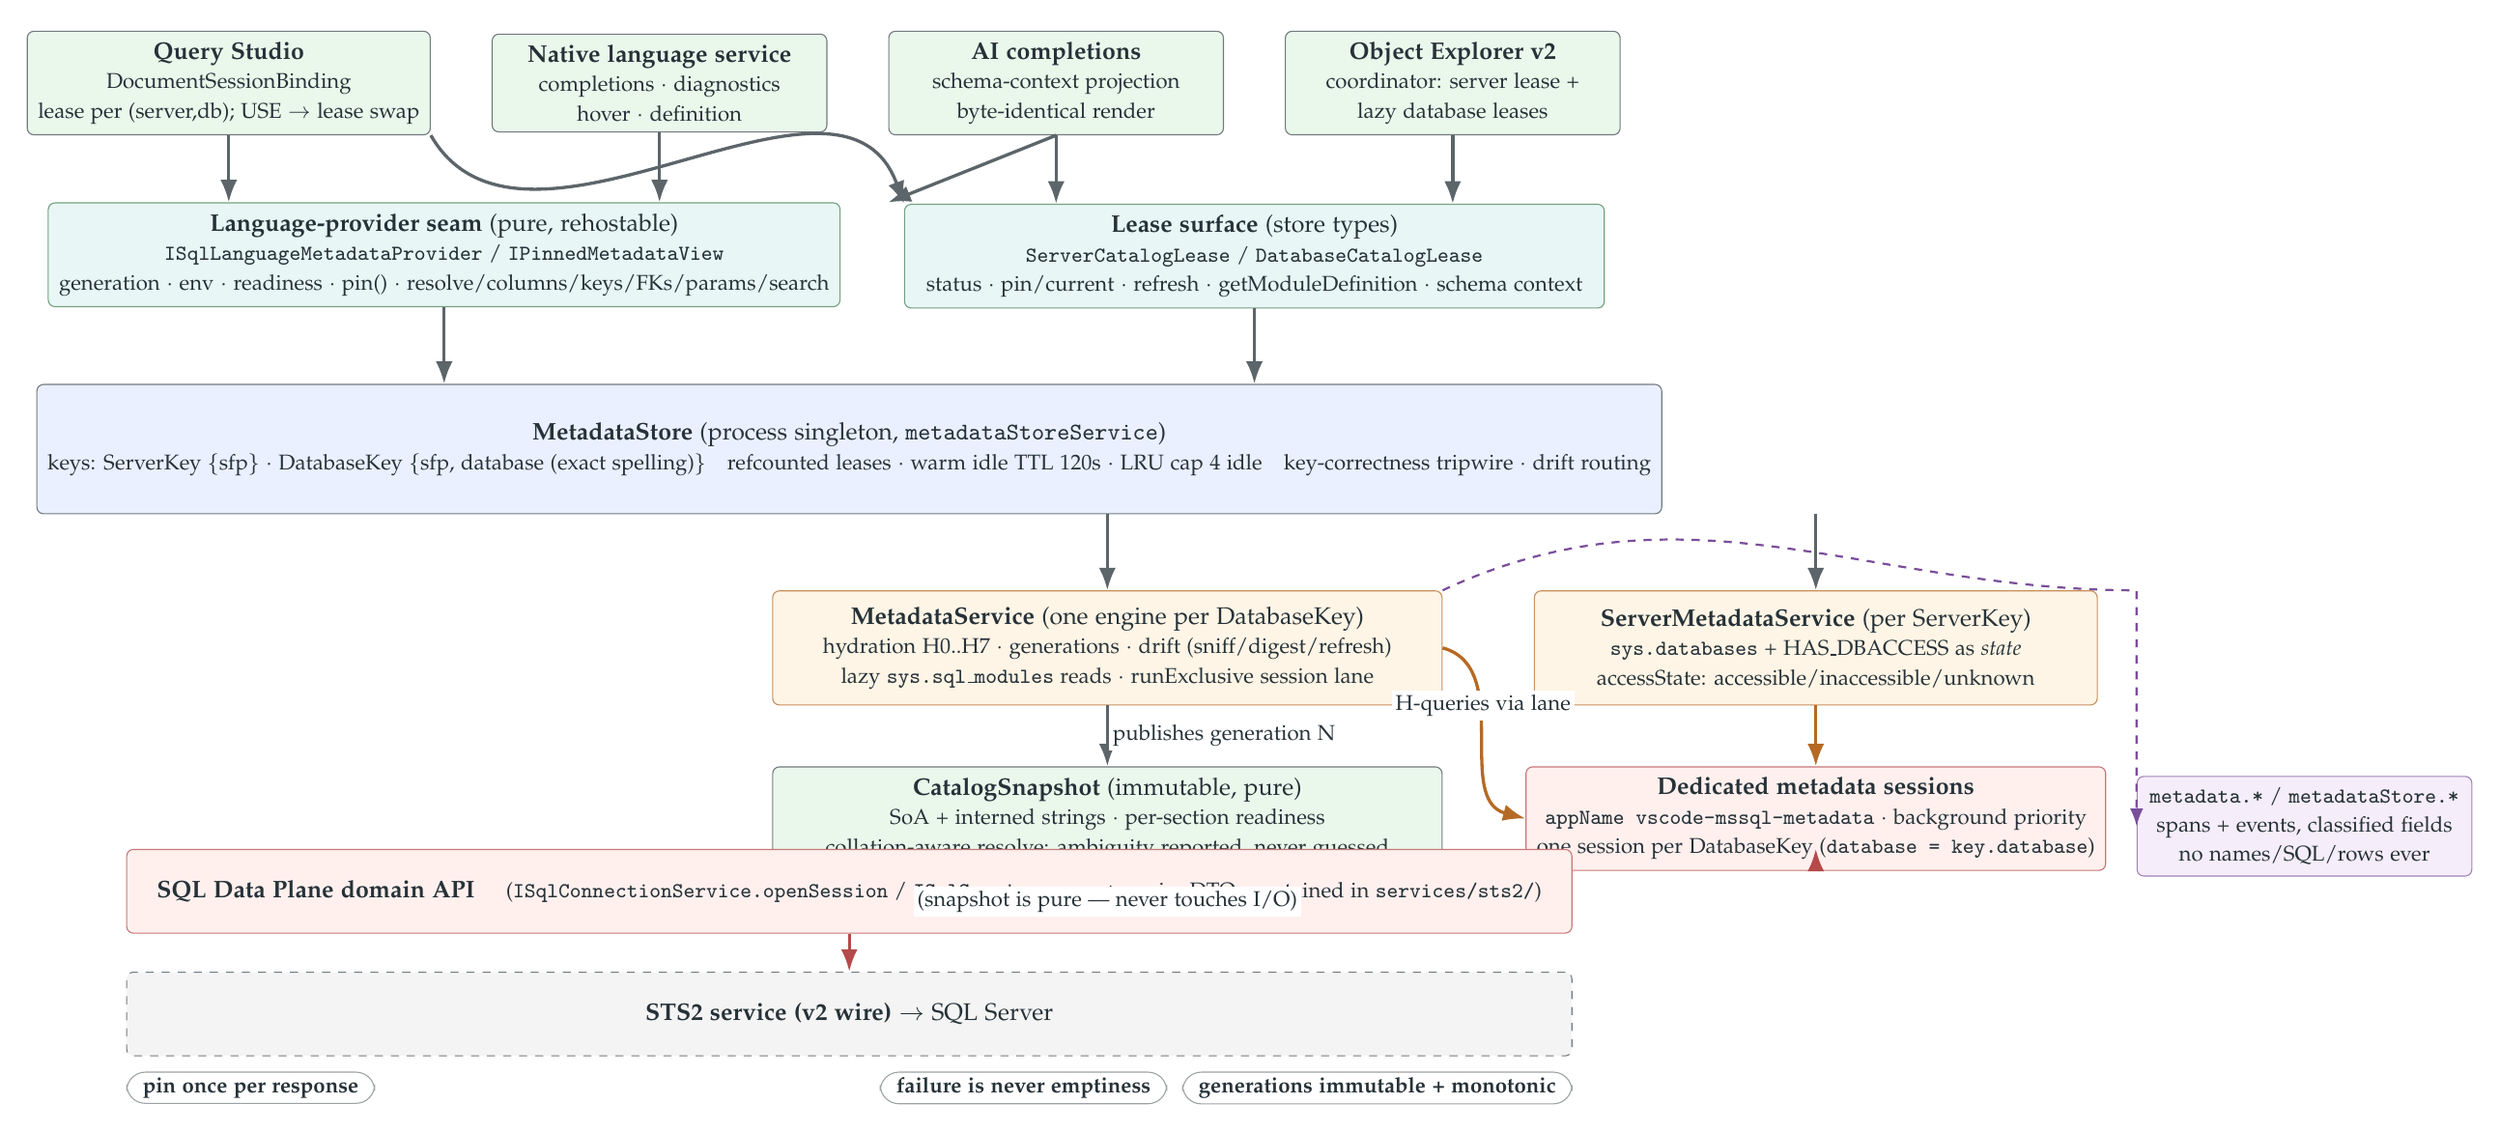
\begin{tikzpicture}[node distance=6mm and 8mm]

% consumers row
\node[corebox,minimum width=44mm] (qs) {\textbf{Query Studio}\\\footnotesize DocumentSessionBinding\\\footnotesize lease per (server,db); USE $\to$ lease swap};
\node[corebox,minimum width=44mm,right=of qs] (ls) {\textbf{Native language service}\\\footnotesize completions $\cdot$ diagnostics\\\footnotesize hover $\cdot$ definition};
\node[corebox,minimum width=44mm,right=of ls] (ai) {\textbf{AI completions}\\\footnotesize schema-context projection\\\footnotesize byte-identical render};
\node[corebox,minimum width=44mm,right=of ai] (oe) {\textbf{Object Explorer v2}\\\footnotesize coordinator: server lease +\\\footnotesize lazy database leases};

% seams
\node[policybox,minimum width=92mm,below=9mm of $(qs.south)!0.5!(ls.south)$] (seam1) {\textbf{Language-provider seam} (pure, rehostable)\\\footnotesize \code{ISqlLanguageMetadataProvider} / \code{IPinnedMetadataView}\\\footnotesize generation $\cdot$ env $\cdot$ readiness $\cdot$ pin() $\cdot$ resolve/columns/keys/FKs/params/search};
\node[policybox,minimum width=92mm,below=9mm of $(ai.south)!0.5!(oe.south)$] (seam2) {\textbf{Lease surface} (store types)\\\footnotesize \code{ServerCatalogLease} / \code{DatabaseCatalogLease}\\\footnotesize status $\cdot$ pin/current $\cdot$ refresh $\cdot$ getModuleDefinition $\cdot$ schema context};

% store layer
\node[box,minimum width=190mm,minimum height=17mm,below=10mm of $(seam1.south)!0.5!(seam2.south)$] (store)
{\textbf{MetadataStore} (process singleton, \code{metadataStoreService})\\\footnotesize
keys: ServerKey \{sfp\} $\cdot$ DatabaseKey \{sfp, database (exact spelling)\}\quad
refcounted leases $\cdot$ warm idle TTL 120s $\cdot$ LRU cap 4 idle\quad
key-correctness tripwire $\cdot$ drift routing};

% engine layer
\node[enginebox,minimum width=88mm,minimum height=15mm,below left=10mm and -78mm of store.south] (dbeng)
{\textbf{MetadataService} (one engine per DatabaseKey)\\\footnotesize hydration H0..H7 $\cdot$ generations $\cdot$ drift (sniff/digest/refresh)\\\footnotesize lazy \code{sys.sql\_modules} reads $\cdot$ runExclusive session lane};
\node[enginebox,minimum width=74mm,minimum height=15mm,right=12mm of dbeng] (srveng)
{\textbf{ServerMetadataService} (per ServerKey)\\\footnotesize \code{sys.databases} + HAS\_DBACCESS as \emph{state}\\\footnotesize accessState: accessible/inaccessible/unknown};

% snapshot
\node[corebox,minimum width=88mm,minimum height=13mm,below=8mm of dbeng] (snap)
{\textbf{CatalogSnapshot} (immutable, pure)\\\footnotesize SoA + interned strings $\cdot$ per-section readiness\\\footnotesize collation-aware resolve: ambiguity reported, never guessed};

% sessions
\node[sessbox,minimum width=74mm,minimum height=13mm,below=8mm of srveng] (sess)
{\textbf{Dedicated metadata sessions}\\\footnotesize \code{appName vscode-mssql-metadata} $\cdot$ background priority\\\footnotesize one session per DatabaseKey (\code{database = key.database})};

% data plane + service
\node[sessbox,minimum width=190mm,minimum height=11mm,below=20mm of store,yshift=-24mm] (dp)
{\textbf{SQL Data Plane domain API} \quad \footnotesize (\code{ISqlConnectionService.openSession} / \code{ISqlSession.execute}; wire DTOs contained in \code{services/sts2/})};
\node[extbox,minimum width=190mm,below=5mm of dp] (sts) {\textbf{STS2 service (v2 wire)} $\to$ SQL Server};

% observability sidecar
\node[obsbox,minimum width=44mm,minimum height=13mm,right=4mm of sess.east,anchor=west,yshift=-1mm] (obs)
{\footnotesize \code{metadata.*} / \code{metadataStore.*}\\\footnotesize spans + events, classified fields\\\footnotesize no names/SQL/rows ever};

% arrows consumers -> seams
\draw[arrow] (qs.south) -- (seam1.north -| qs.south);
\draw[arrow] (ls.south) -- (seam1.north -| ls.south);
\draw[arrow] (ai.south) -- (seam1.north -| ai.south west);
\draw[arrow] (ai.south) -- (seam2.north -| ai.south);
\draw[arrow] (oe.south) -- (seam2.north -| oe.south);
\draw[arrow] (qs.south east) to[out=-60,in=110] (seam2.north west);

% seams -> store
\draw[arrow] (seam1.south) -- (store.north -| seam1.south);
\draw[arrow] (seam2.south) -- (store.north -| seam2.south);

% store -> engines
\draw[arrow] (store.south -| dbeng.north) -- (dbeng.north);
\draw[arrow] (store.south -| srveng.north) -- (srveng.north);

% engines -> snapshot / sessions
\draw[arrow] (dbeng.south) -- node[label,right]{publishes generation N} (snap.north);
\draw[effect] (dbeng.east) to[out=-15,in=165] node[label,above,pos=0.45]{H-queries via lane} (sess.west);
\draw[effect] (srveng.south) -- (sess.north -| srveng.south);

% sessions -> dp -> sts
\draw[write] (sess.south) -- (dp.north -| sess.south);
\node[label,below=2mm of snap.south]{\footnotesize (snapshot is pure --- never touches I/O)};
\draw[write] (dp.south) -- (sts.north);

% obs
\draw[async] (dbeng.north east) to[out=25,in=180] (obs.west |- dbeng.north east) -- (obs.west);

% invariant pills
\node[pill,below=2mm of sts.south west,anchor=north west] {pin once per response};
\node[pill,right=4mm of sts.south,anchor=north west,yshift=-2mm] {failure is never emptiness};
\node[pill,below=2mm of sts.south east,anchor=north east] {generations immutable + monotonic};

\end{tikzpicture}
\end{adjustbox}

\newpage
% =====================================================================
% PAGE 2 — KEYS AND LEASE LIFECYCLE
% =====================================================================
\pagehead{2. Identity, key-correctness, and the lease lifecycle}
{Hash fingerprints (never reversible), per-database sessions keyed by construction, and the warm TTL + LRU entry state machine.}
\legend\par\vspace{4mm}

\begin{adjustbox}{max width=\linewidth,max height=0.82\textheight,center}
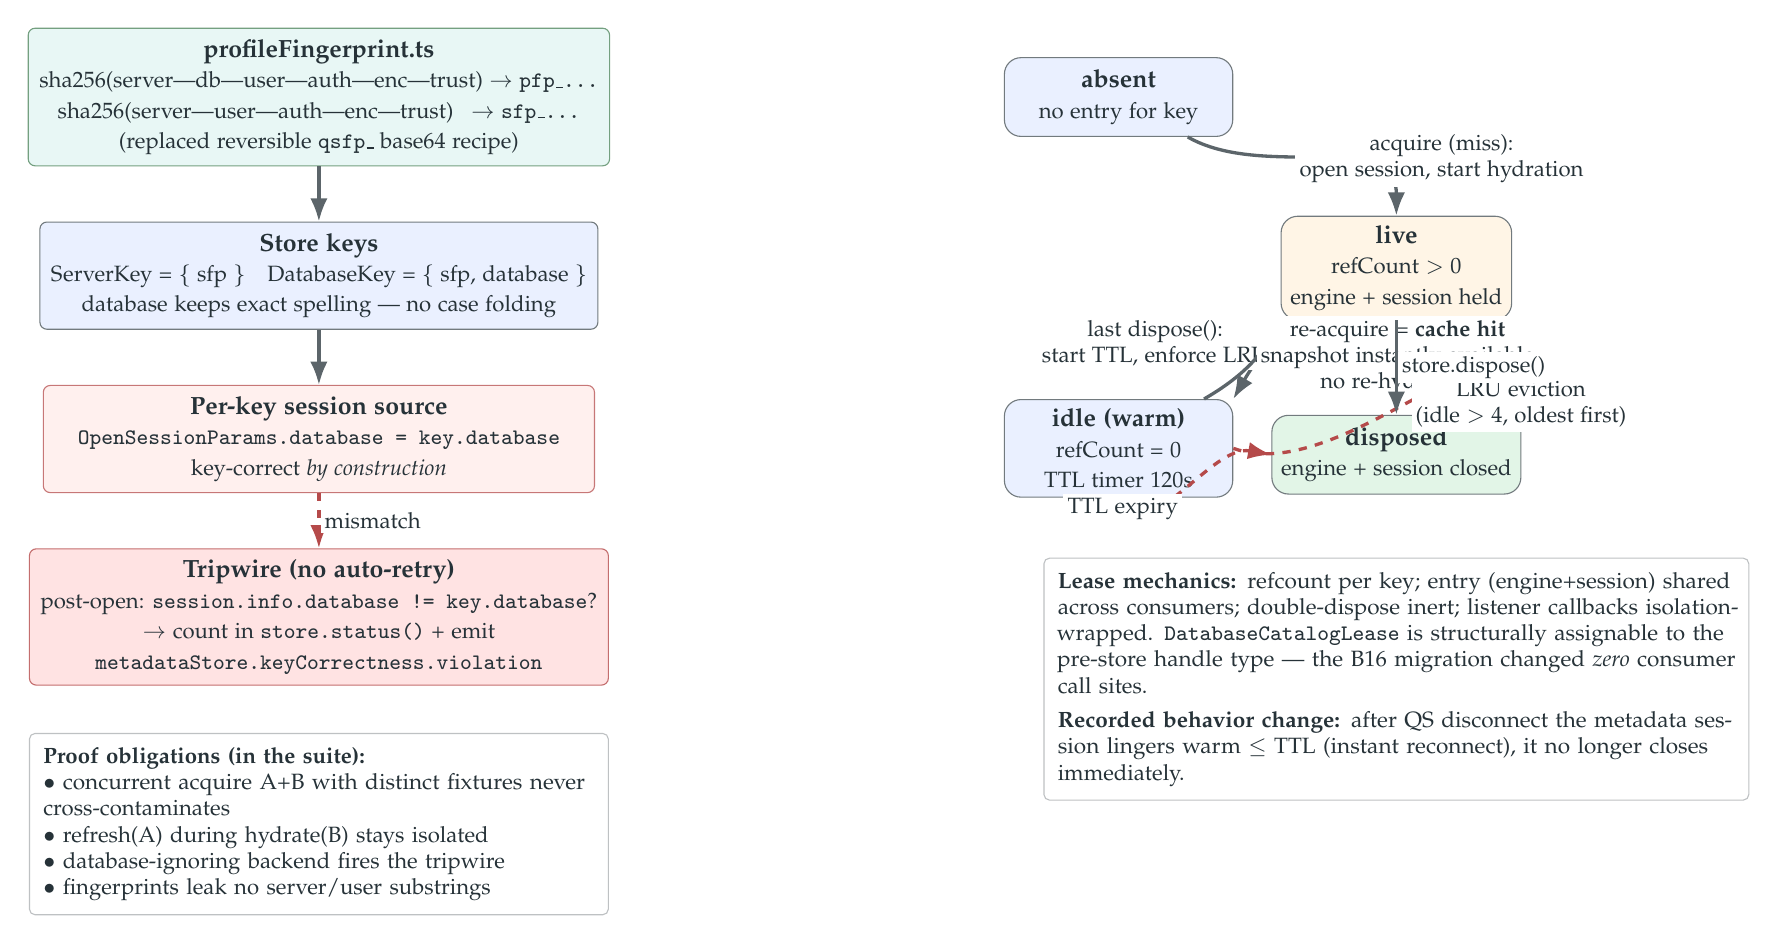
\begin{tikzpicture}[node distance=7mm and 10mm]

% --- left column: identity
\node[policybox,minimum width=70mm,minimum height=16mm] (fp)
{\textbf{profileFingerprint.ts}\\\footnotesize sha256(server|db|user|auth|enc|trust) $\to$ \code{pfp\_...}\\\footnotesize sha256(server|user|auth|enc|trust) \enspace$\to$ \code{sfp\_...}\\\footnotesize (replaced reversible \code{qsfp\_} base64 recipe)};
\node[box,minimum width=70mm,below=of fp] (keys)
{\textbf{Store keys}\\\footnotesize ServerKey = \{ sfp \}\quad DatabaseKey = \{ sfp, database \}\\\footnotesize database keeps exact spelling --- no case folding};
\node[sessbox,minimum width=70mm,below=of keys] (src)
{\textbf{Per-key session source}\\\footnotesize \code{OpenSessionParams.database = key.database}\\\footnotesize key-correct \emph{by construction}};
\node[riskbox,minimum width=70mm,below=of src] (trip)
{\textbf{Tripwire (no auto-retry)}\\\footnotesize post-open: \code{session.info.database != key.database}?\\\footnotesize $\to$ count in \code{store.status()} + emit\\\footnotesize \code{metadataStore.keyCorrectness.violation}};
\draw[arrow] (fp) -- (keys);
\draw[arrow] (keys) -- (src);
\draw[fail] (src) -- node[label,right]{mismatch} (trip);

\node[note,below=6mm of trip,text width=70mm] (proof)
{\textbf{Proof obligations (in the suite):}\\
$\bullet$ concurrent acquire A+B with distinct fixtures never cross-contaminates\\
$\bullet$ refresh(A) during hydrate(B) stays isolated\\
$\bullet$ database-ignoring backend fires the tripwire\\
$\bullet$ fingerprints leak no server/user substrings};

% --- right: lease entry state machine
\node[state,right=34mm of fp,xshift=16mm] (absent) {\textbf{absent}\\\footnotesize no entry for key};
\node[state,fill=edge,below right=10mm and 6mm of absent] (live) {\textbf{live}\\\footnotesize refCount $>$ 0\\\footnotesize engine + session held};
\node[state,below left=10mm and 6mm of live] (idle) {\textbf{idle (warm)}\\\footnotesize refCount = 0\\\footnotesize TTL timer 120s};
\node[term,below=12mm of live] (disposed) {\textbf{disposed}\\\footnotesize engine + session closed};

\draw[arrow] (absent) to[out=-30,in=90] node[label,right,pos=0.4]{acquire (miss):\\\footnotesize open session, start hydration} (live.north);
\draw[arrow] (live) to[out=-150,in=60] node[label,left,pos=0.35]{last dispose():\\\footnotesize start TTL, enforce LRU} (idle.north east);
\draw[arrow] (idle) to[out=30,in=-120] node[label,right,pos=0.6]{re-acquire = \textbf{cache hit}\\\footnotesize snapshot instantly available\\\footnotesize no re-hydration} (live.south west);
\draw[fail] (idle.south) to[out=-60,in=170] node[label,below left]{TTL expiry} (disposed.west);
\draw[fail] (idle.east) to[out=-20,in=100] node[label,right]{LRU eviction\\\footnotesize (idle $>$ 4, oldest first)} (disposed.north east);
\draw[arrow] (live) -- node[label,right]{store.dispose()} (disposed);

\node[note,below=8mm of disposed,text width=86mm]
{\textbf{Lease mechanics:} refcount per key; entry (engine+session) shared across consumers; double-dispose inert; listener callbacks isolation-wrapped. \code{DatabaseCatalogLease} is structurally assignable to the pre-store handle type --- the B16 migration changed \emph{zero} consumer call sites.\\[1mm]
\textbf{Recorded behavior change:} after QS disconnect the metadata session lingers warm $\le$ TTL (instant reconnect), it no longer closes immediately.};

\end{tikzpicture}
\end{adjustbox}

\newpage
% =====================================================================
% PAGE 3 — HYDRATION, GENERATIONS, DRIFT
% =====================================================================
\pagehead{3. Hydration ladder, generations, and the drift loop}
{H0--H7 over the serialized session lane; forced refreshes chain (never overlap); three drift triggers, cheapest first.}
\legend\par\vspace{4mm}

\begin{adjustbox}{max width=\linewidth,max height=0.82\textheight,center}
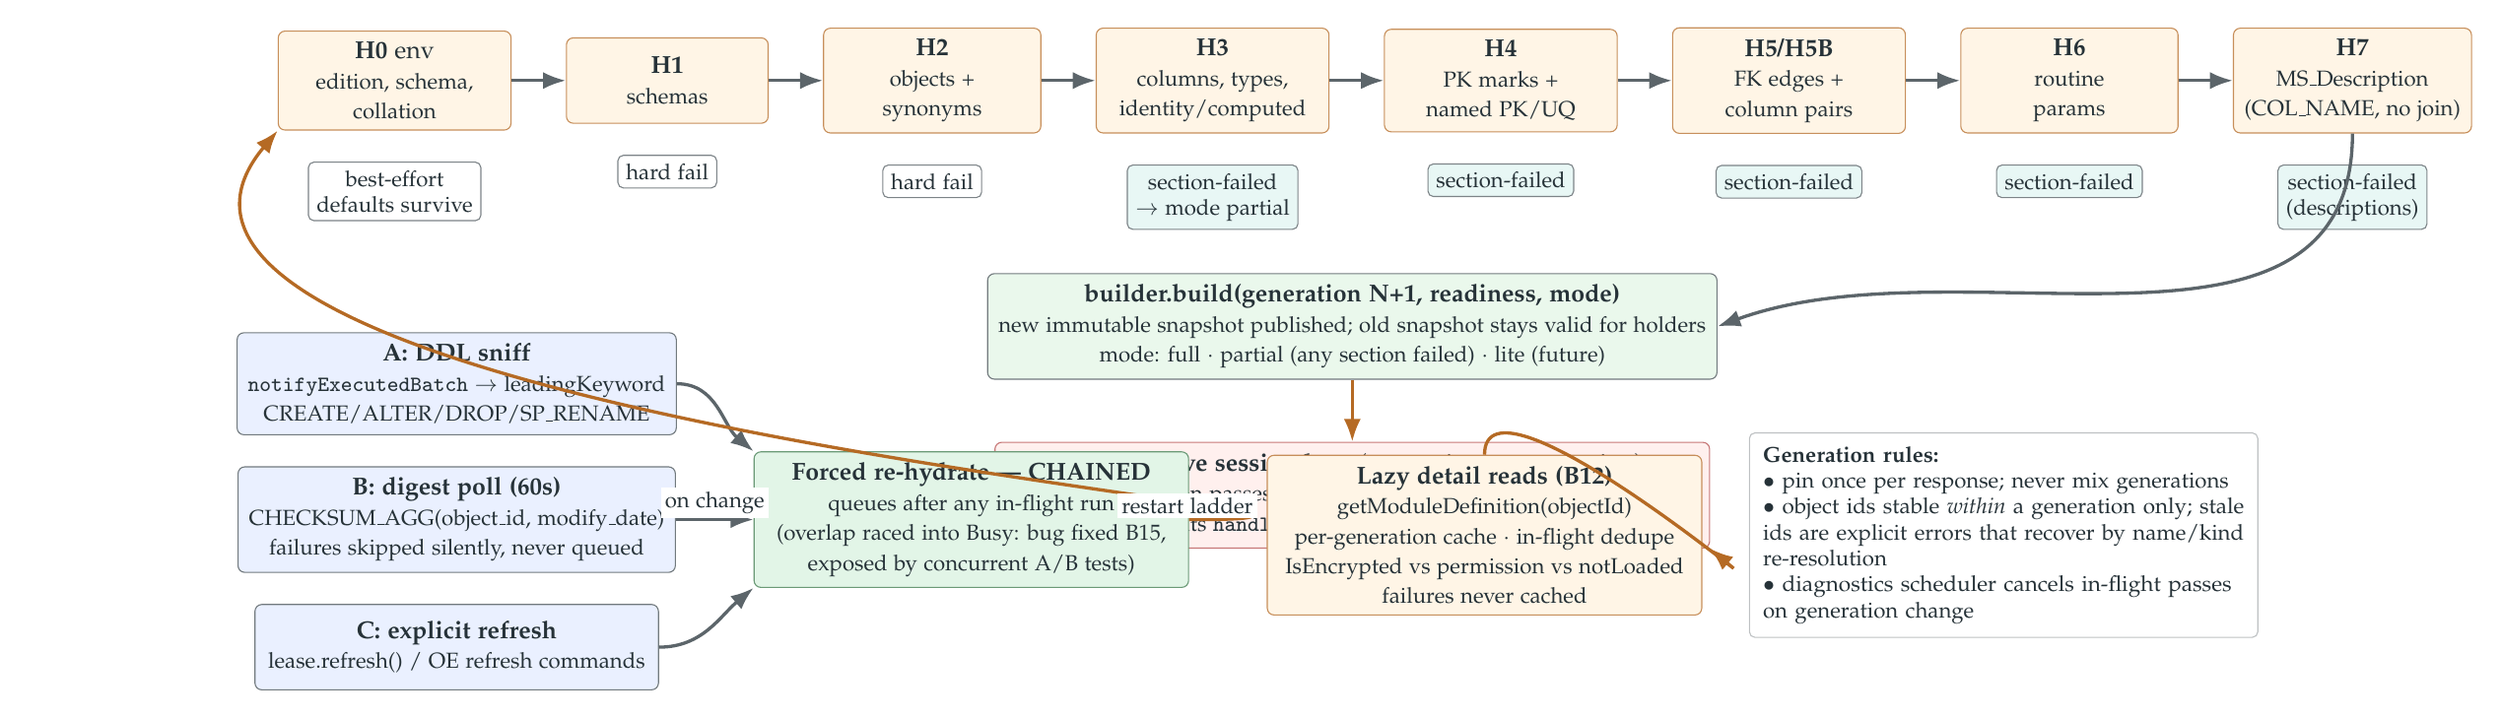
\begin{tikzpicture}[node distance=5mm and 7mm]

% ladder
\node[enginebox,minimum width=30mm] (h0) {\textbf{H0} env\\\footnotesize edition, schema,\\\footnotesize collation};
\node[enginebox,minimum width=26mm,right=of h0] (h1) {\textbf{H1}\\\footnotesize schemas};
\node[enginebox,minimum width=28mm,right=of h1] (h2) {\textbf{H2}\\\footnotesize objects +\\\footnotesize synonyms};
\node[enginebox,minimum width=30mm,right=of h2] (h3) {\textbf{H3}\\\footnotesize columns, types,\\\footnotesize identity/computed};
\node[enginebox,minimum width=30mm,right=of h3] (h4) {\textbf{H4}\\\footnotesize PK marks +\\\footnotesize named PK/UQ};
\node[enginebox,minimum width=30mm,right=of h4] (h5) {\textbf{H5/H5B}\\\footnotesize FK edges +\\\footnotesize column pairs};
\node[enginebox,minimum width=28mm,right=of h5] (h6) {\textbf{H6}\\\footnotesize routine\\\footnotesize params};
\node[enginebox,minimum width=30mm,right=of h6] (h7) {\textbf{H7}\\\footnotesize MS\_Description\\\footnotesize (COL\_NAME, no join)};

\draw[arrow] (h0) -- (h1);
\draw[arrow] (h1) -- (h2);
\draw[arrow] (h2) -- (h3);
\draw[arrow] (h3) -- (h4);
\draw[arrow] (h4) -- (h5);
\draw[arrow] (h5) -- (h6);
\draw[arrow] (h6) -- (h7);

% failure policies
\node[tinybox,below=4mm of h0] {best-effort\\defaults survive};
\node[tinybox,below=4mm of h1] {hard fail};
\node[tinybox,below=4mm of h2] {hard fail};
\node[tinybox,below=4mm of h3,fill=policy] {section-failed\\$\to$ mode partial};
\node[tinybox,below=4mm of h4,fill=policy] {section-failed};
\node[tinybox,below=4mm of h5,fill=policy] {section-failed};
\node[tinybox,below=4mm of h6,fill=policy] {section-failed};
\node[tinybox,below=4mm of h7,fill=policy] {section-failed\\(descriptions)};

% generation publish
\node[corebox,minimum width=86mm,below=18mm of h3.south,xshift=18mm] (gen)
{\textbf{builder.build(generation N+1, readiness, mode)}\\\footnotesize new immutable snapshot published; old snapshot stays valid for holders\\\footnotesize mode: full $\cdot$ partial (any section failed) $\cdot$ lite (future)};
\draw[arrow] (h7.south) to[out=-90,in=20] (gen.east);

% lane
\node[sessbox,minimum width=86mm,below=8mm of gen] (lane)
{\textbf{runExclusive session lane} (one-active-query session)\\\footnotesize serializes: hydration passes $\cdot$ digest polls $\cdot$ lazy \code{sys.sql\_modules} reads\\\footnotesize every query awaits \code{handle.completion} (reaction-order slot release)};
\draw[effect] (gen.south) -- (lane.north);

% drift loop (left cluster)
\node[box,minimum width=52mm,below=26mm of h0.south,xshift=8mm] (sniff)
{\textbf{A: DDL sniff}\\\footnotesize \code{notifyExecutedBatch} $\to$ leadingKeyword\\\footnotesize CREATE/ALTER/DROP/SP\_RENAME};
\node[box,minimum width=52mm,below=4mm of sniff] (digest)
{\textbf{B: digest poll (60s)}\\\footnotesize CHECKSUM\_AGG(object\_id, modify\_date)\\\footnotesize failures skipped silently, never queued};
\node[box,minimum width=52mm,below=4mm of digest] (explicit)
{\textbf{C: explicit refresh}\\\footnotesize lease.refresh() / OE refresh commands};

\node[goodbox,minimum width=56mm,right=10mm of digest] (chain)
{\textbf{Forced re-hydrate --- CHAINED}\\\footnotesize queues after any in-flight run\\\footnotesize (overlap raced into Busy: bug fixed B15,\\\footnotesize exposed by concurrent A/B tests)};

\draw[arrow] (sniff.east) to[out=0,in=140] (chain.north west);
\draw[arrow] (digest.east) -- node[label,above]{on change} (chain.west);
\draw[arrow] (explicit.east) to[out=0,in=-140] (chain.south west);
\draw[effect] (chain.east) to[out=0,in=-130] node[label,below right,pos=0.3]{restart ladder} (h0.south west);

% lazy reads
\node[enginebox,minimum width=56mm,right=10mm of chain,yshift=-2mm] (lazy)
{\textbf{Lazy detail reads (B12)}\\\footnotesize getModuleDefinition(objectId)\\\footnotesize per-generation cache $\cdot$ in-flight dedupe\\\footnotesize IsEncrypted vs permission vs notLoaded\\\footnotesize failures never cached};
\draw[effect] (lazy.north) to[out=90,in=-40] (lane.south east);

\node[note,right=6mm of lazy,text width=62mm]
{\textbf{Generation rules:}\\
$\bullet$ pin once per response; never mix generations\\
$\bullet$ object ids stable \emph{within} a generation only; stale ids are explicit errors that recover by name/kind re-resolution\\
$\bullet$ diagnostics scheduler cancels in-flight passes on generation change};

\end{tikzpicture}
\end{adjustbox}

\newpage
% =====================================================================
% PAGE 4 — CONSUMER FLOWS + PRIVACY GATES
% =====================================================================
\pagehead{4. Consumer data flows and the privacy gates}
{The same snapshot serves four masters; what may leave each boundary is classified, tested, and canaried.}
\legend\par\vspace{4mm}

\begin{adjustbox}{max width=\linewidth,max height=0.82\textheight,center}
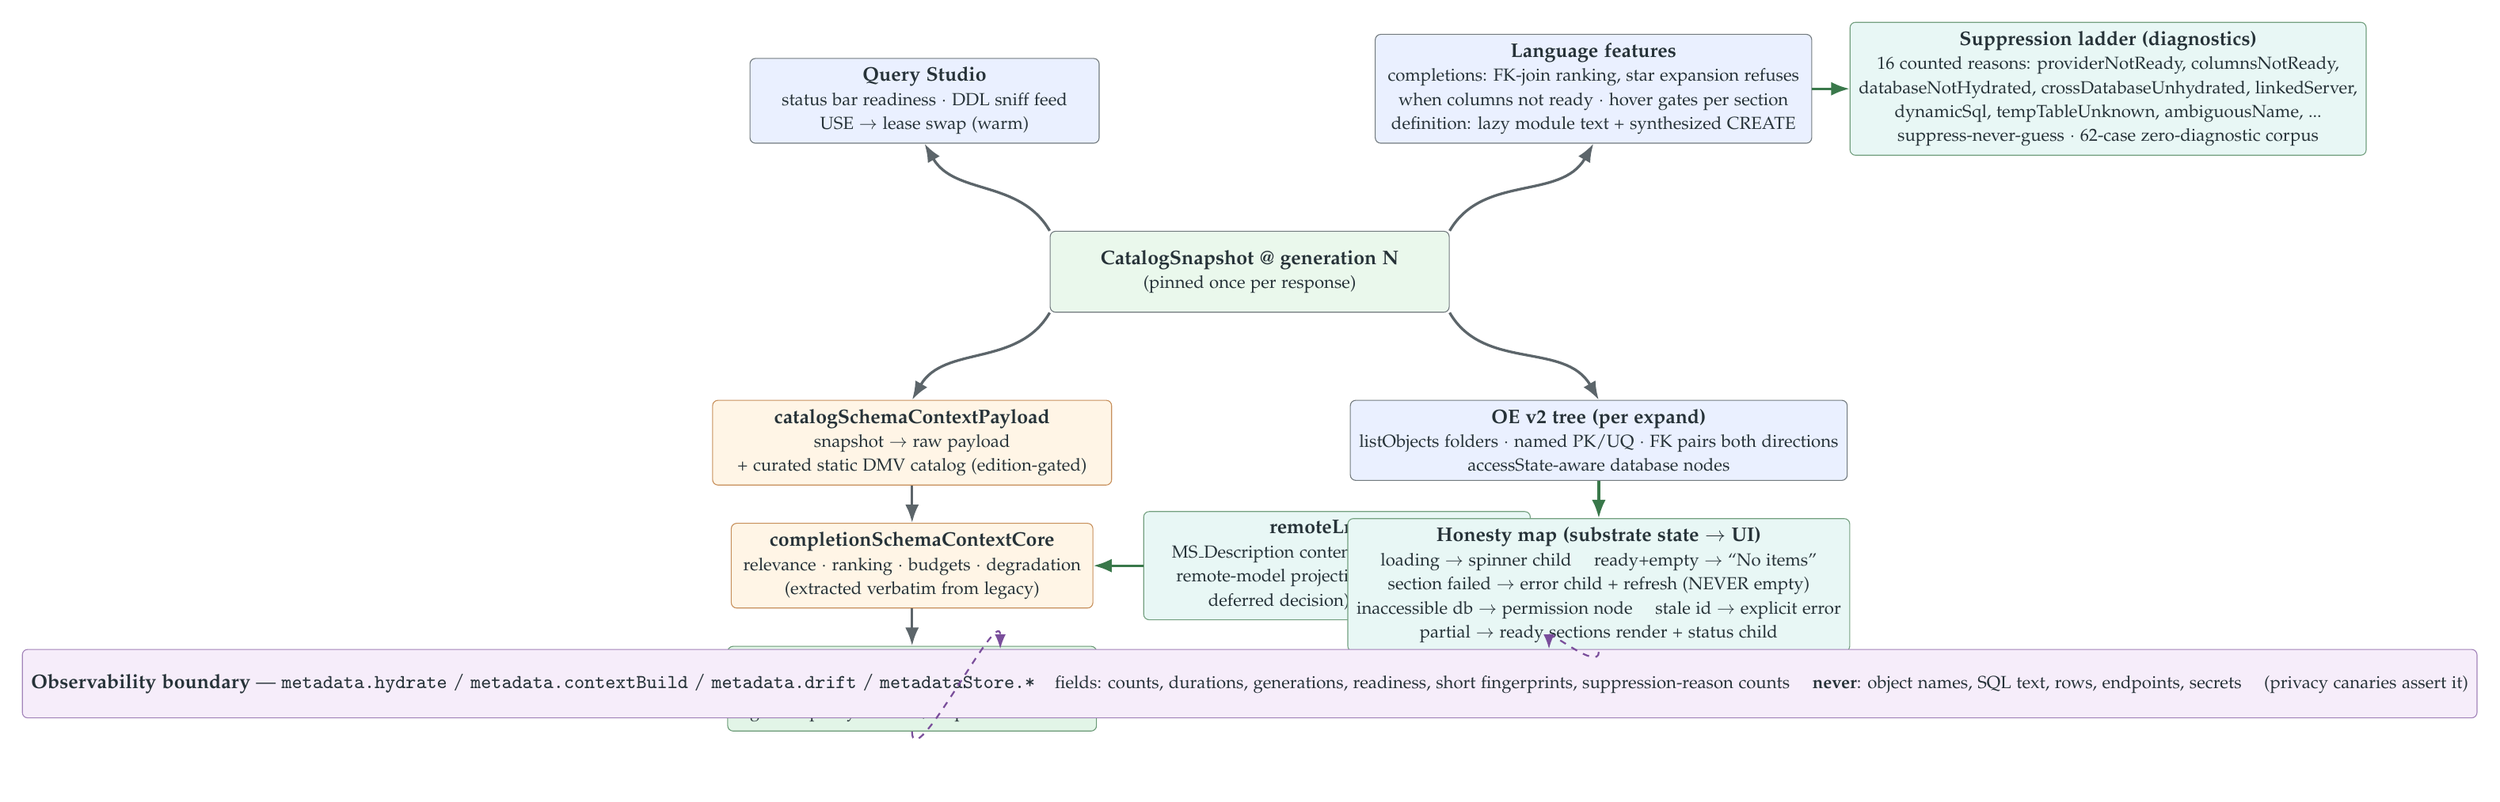
\begin{tikzpicture}[node distance=6mm and 9mm]

\node[corebox,minimum width=64mm,minimum height=13mm] (snap)
{\textbf{CatalogSnapshot @ generation N}\\\footnotesize (pinned once per response)};

% QS flow
\node[box,minimum width=56mm,above left=14mm and -8mm of snap] (qs)
{\textbf{Query Studio}\\\footnotesize status bar readiness $\cdot$ DDL sniff feed\\\footnotesize USE $\to$ lease swap (warm)};
\draw[arrow] (snap.north west) to[out=120,in=-60] (qs.south);

% LS flow
\node[box,minimum width=70mm,above right=14mm and -12mm of snap] (ls)
{\textbf{Language features}\\\footnotesize completions: FK-join ranking, star expansion refuses\\\footnotesize when columns not ready $\cdot$ hover gates per section\\\footnotesize definition: lazy module text + synthesized CREATE};
\draw[arrow] (snap.north east) to[out=60,in=-120] (ls.south);

\node[policybox,minimum width=70mm,right=6mm of ls,anchor=west,yshift=0mm] (ladder)
{\textbf{Suppression ladder (diagnostics)}\\\footnotesize 16 counted reasons: providerNotReady, columnsNotReady,\\\footnotesize databaseNotHydrated, crossDatabaseUnhydrated, linkedServer,\\\footnotesize dynamicSql, tempTableUnknown, ambiguousName, ...\\\footnotesize suppress-never-guess $\cdot$ 62-case zero-diagnostic corpus};
\draw[policyarr] (ls.east) -- (ladder.west);

% AI flow
\node[enginebox,minimum width=64mm,below left=14mm and -10mm of snap] (payload)
{\textbf{catalogSchemaContextPayload}\\\footnotesize snapshot $\to$ raw payload\\\footnotesize + curated static DMV catalog (edition-gated)};
\node[enginebox,minimum width=58mm,below=6mm of payload] (corepipe)
{\textbf{completionSchemaContextCore}\\\footnotesize relevance $\cdot$ ranking $\cdot$ budgets $\cdot$ degradation\\\footnotesize (extracted verbatim from legacy)};
\node[goodbox,minimum width=58mm,below=6mm of corepipe] (bytes)
{\textbf{buildSchemaContext render}\\\footnotesize \textbf{BYTE-IDENTICAL} per (generation, request)\\\footnotesize golden-parity suite 10/10 pins exact lines};
\draw[arrow] (snap.south west) to[out=-120,in=60] (payload.north);
\draw[arrow] (payload) -- (corepipe);
\draw[arrow] (corepipe) -- (bytes);

\node[policybox,minimum width=62mm,right=8mm of corepipe]
(gate1)
{\textbf{remoteLm gate}\\\footnotesize MS\_Description content EXCLUDED from\\\footnotesize remote-model projections (one-way door,\\\footnotesize deferred decision) --- test-pinned};
\draw[policyarr] (gate1.west) -- (corepipe.east);

% OE flow
\node[box,minimum width=74mm,below right=14mm and -16mm of snap] (oe)
{\textbf{OE v2 tree (per expand)}\\\footnotesize listObjects folders $\cdot$ named PK/UQ $\cdot$ FK pairs both directions\\\footnotesize accessState-aware database nodes};
\draw[arrow] (snap.south east) to[out=-60,in=120] (oe.north);

\node[policybox,minimum width=74mm,below=6mm of oe] (honesty)
{\textbf{Honesty map (substrate state $\to$ UI)}\\\footnotesize loading $\to$ spinner child \quad ready+empty $\to$ ``No items''\\\footnotesize section failed $\to$ error child + refresh (NEVER empty)\\\footnotesize inaccessible db $\to$ permission node \quad stale id $\to$ explicit error\\\footnotesize partial $\to$ ready sections render + status child};
\draw[policyarr] (oe) -- (honesty);

% observability strip
\node[obsbox,minimum width=178mm,below=30mm of snap,yshift=-24mm] (obs)
{\textbf{Observability boundary} --- \code{metadata.hydrate} / \code{metadata.contextBuild} / \code{metadata.drift} / \code{metadataStore.*}\quad
\footnotesize fields: counts, durations, generations, readiness, short fingerprints, suppression-reason counts \quad
\textbf{never}: object names, SQL text, rows, endpoints, secrets \quad (privacy canaries assert it)};
\draw[async] (bytes.south) to[out=-90,in=90] ([xshift=-40mm]obs.north);
\draw[async] (honesty.south) to[out=-90,in=90] ([xshift=48mm]obs.north);

\end{tikzpicture}
\end{adjustbox}

\newpage
% =====================================================================
% PAGE 5 — SESSION STRATEGY AND MEASURED NUMBERS
% =====================================================================
\pagehead{5. Session strategy, alternatives, and measured performance}
{Why per-database dedicated sessions won the preview; what would trigger the serialized-USE lane; the numbers that hold it all up.}
\legend\par\vspace{4mm}

\begin{adjustbox}{max width=\linewidth,max height=0.82\textheight,center}
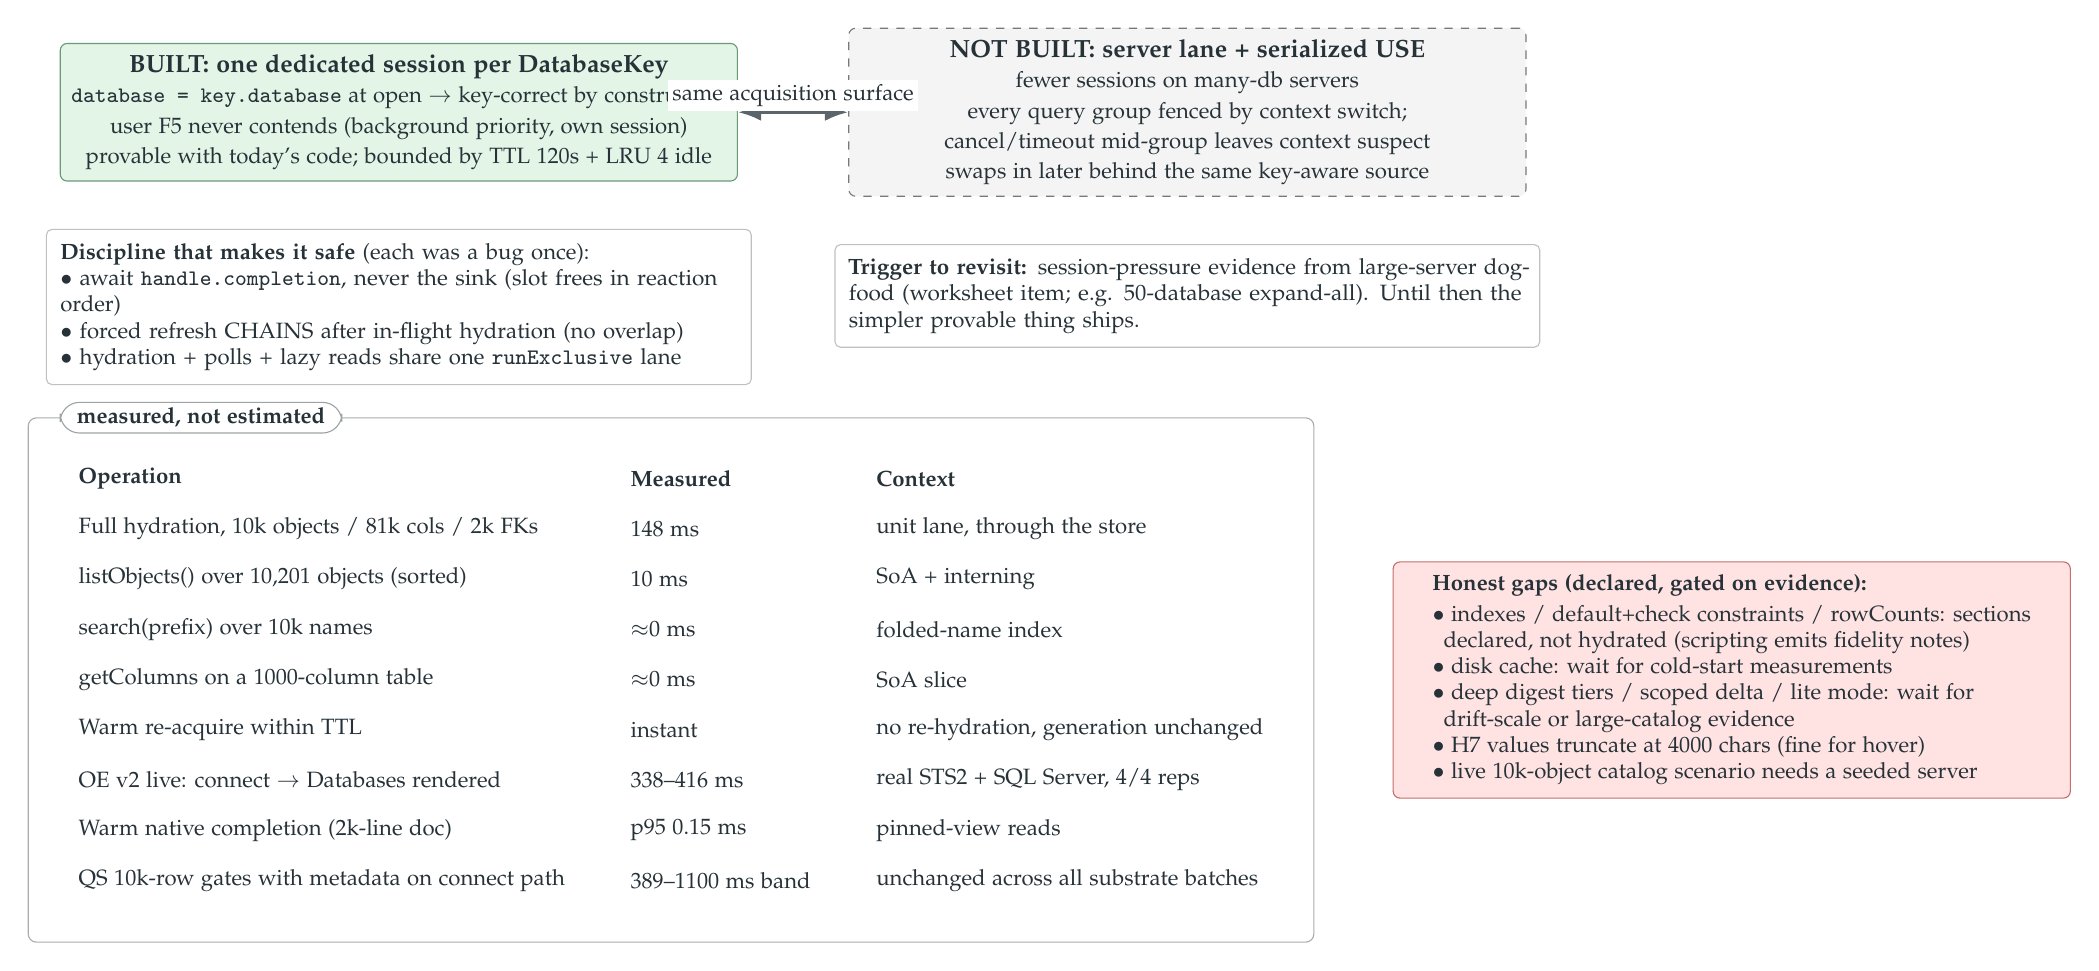
\begin{tikzpicture}[node distance=6mm and 10mm]

% chosen strategy
\node[goodbox,minimum width=86mm,minimum height=17mm] (chosen)
{\textbf{BUILT: one dedicated session per DatabaseKey}\\\footnotesize \code{database = key.database} at open $\to$ key-correct by construction\\\footnotesize user F5 never contends (background priority, own session)\\\footnotesize provable with today's code; bounded by TTL 120s + LRU 4 idle};

\node[extbox,minimum width=86mm,minimum height=17mm,right=14mm of chosen] (alt)
{\textbf{NOT BUILT: server lane + serialized USE}\\\footnotesize fewer sessions on many-db servers\\\footnotesize every query group fenced by context switch;\\\footnotesize cancel/timeout mid-group leaves context suspect\\\footnotesize swaps in later behind the same key-aware source};

\draw[arrow,<->] (chosen) -- node[label,above]{same acquisition surface} (alt);

\node[note,below=6mm of chosen,text width=86mm]
{\textbf{Discipline that makes it safe} (each was a bug once):\\
$\bullet$ await \code{handle.completion}, never the sink (slot frees in reaction order)\\
$\bullet$ forced refresh CHAINS after in-flight hydration (no overlap)\\
$\bullet$ hydration + polls + lazy reads share one \code{runExclusive} lane};

\node[note,below=6mm of alt,text width=86mm]
{\textbf{Trigger to revisit:} session-pressure evidence from large-server dogfood (worksheet item; e.g. 50-database expand-all). Until then the simpler provable thing ships.};

% measured numbers table
\matrix (perf) [matrix of nodes,below=34mm of chosen.south west,anchor=north west,xshift=0mm,
  row sep=1.2mm,column sep=6mm,
  nodes={font=\footnotesize,anchor=west},
  row 1/.style={nodes={font=\footnotesize\bfseries}}]
{
Operation & Measured & Context \\
Full hydration, 10k objects / 81k cols / 2k FKs & 148 ms & unit lane, through the store \\
listObjects() over 10{,}201 objects (sorted) & 10 ms & SoA + interning \\
search(prefix) over 10k names & $\approx$0 ms & folded-name index \\
getColumns on a 1000-column table & $\approx$0 ms & SoA slice \\
Warm re-acquire within TTL & instant & no re-hydration, generation unchanged \\
OE v2 live: connect $\to$ Databases rendered & 338--416 ms & real STS2 + SQL Server, 4/4 reps \\
Warm native completion (2k-line doc) & p95 0.15 ms & pinned-view reads \\
QS 10k-row gates with metadata on connect path & 389--1100 ms band & unchanged across all substrate batches \\
};
\begin{scope}[on background layer]
\node[draw=ink!40,rounded corners=3pt,fill=white,fit=(perf),inner sep=4mm] {};
\end{scope}
\node[pill,anchor=south west] at ([yshift=2mm]perf.north west) {measured, not estimated};

% gaps box
\node[riskbox,minimum width=86mm,minimum height=30mm,right=14mm of perf.east,anchor=west,align=left,font=\footnotesize]
(gaps)
{\textbf{Honest gaps (declared, gated on evidence):}\\[0.5mm]
$\bullet$ indexes / default+check constraints / rowCounts: sections\\
\enspace declared, not hydrated (scripting emits fidelity notes)\\
$\bullet$ disk cache: wait for cold-start measurements\\
$\bullet$ deep digest tiers / scoped delta / lite mode: wait for\\
\enspace drift-scale or large-catalog evidence\\
$\bullet$ H7 values truncate at 4000 chars (fine for hover)\\
$\bullet$ live 10k-object catalog scenario needs a seeded server};

\end{tikzpicture}
\end{adjustbox}

\end{document}
